\section{Despre proiect}
Un calculator software este un calculator care a fost implementat ca un program, în loc să fie un dispozitiv hardware fizic dedicat acestui scop.

\subsection{Cum arată?}
\begin{figure}[H]
 \begin{center}
  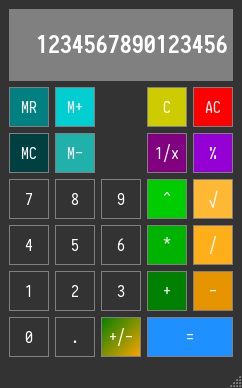
\includegraphics[scale=1.2]{calculator}
 \end{center}
 \caption{Interfața calculatorului}
 \label{fig: Interfața programului}
\end{figure}

Am creat o interfață colorată pentru ca utilizatorul să poată să deosebească operațiile cu ușurință.
\subsection{Opțiuni}
\begin{itemize}
 \item operațiile de bază:
 \begin{itemize}
  \item adunare ($+$)
  \item scădere ($-$)
  \item înmulțire ($\cdot$)
  \item împărțire ($\div$)
 \end{itemize}
\item funcția exponențială/ridicarea la putere ($x^n$)
\item radicalul/rădăcina pătrată a numărului ($\sqrt{}$)
\item schimbarea semnului ($+$/$-$)
\item inversul numărului ($\frac{1}{x}$)
\item procente ($\%$)
\item funcționalitate de memorie (\texttt{MR/MC/M+/M-})
\end{itemize}


\subsection{De ce am ales acest proiect?}
Motivul pentru care am ales să fac un calculator pentru proiectul de atestat este deoarece calculatorul este unul din cele mai simple, des folosite, dar și indispensabile programe pe care cineva le folosește atunci când utilizează un sistem de calcul.



%\clearpage

